\documentclass[A4paper,draft]{scrreprt}
\usepackage{lmodern}
\usepackage{amssymb,amsmath}
\usepackage{ifxetex,ifluatex}
\usepackage{fixltx2e} % provides \textsubscript
\ifnum 0\ifxetex 1\fi\ifluatex 1\fi=0 % if pdftex
  \usepackage[T1]{fontenc}
  \usepackage[utf8]{inputenc}
\else % if luatex or xelatex
  \ifxetex
    \usepackage{mathspec}
  \else
    \usepackage{fontspec}
  \fi
  \defaultfontfeatures{Ligatures=TeX,Scale=MatchLowercase}
\fi
% use upquote if available, for straight quotes in verbatim environments
\IfFileExists{upquote.sty}{\usepackage{upquote}}{}
% use microtype if available
\IfFileExists{microtype.sty}{%
\usepackage[]{microtype}
\UseMicrotypeSet[protrusion]{basicmath} % disable protrusion for tt fonts
}{}
\PassOptionsToPackage{hyphens}{url} % url is loaded by hyperref
\usepackage[unicode=true]{hyperref}
\PassOptionsToPackage{usenames,dvipsnames}{color} % color is loaded by hyperref
\hypersetup{
            pdftitle={Feature analysis of dual stream convolutional neural networks for egocentric action recognition},
            pdfauthor={Will Price},
            pdfkeywords={cnn, ann, convnet, excitation backprop, visualisation, feature analysis, two stream cnn, action recognition},
            colorlinks=true,
            linkcolor=Maroon,
            citecolor=Blue,
            urlcolor=Blue,
            breaklinks=true}
\urlstyle{same}  % don't use monospace font for urls
\usepackage[margin=1in]{geometry}
\usepackage{graphicx,grffile}
\makeatletter
\def\maxwidth{\ifdim\Gin@nat@width>\linewidth\linewidth\else\Gin@nat@width\fi}
\def\maxheight{\ifdim\Gin@nat@height>\textheight\textheight\else\Gin@nat@height\fi}
\makeatother
% Scale images if necessary, so that they will not overflow the page
% margins by default, and it is still possible to overwrite the defaults
% using explicit options in \includegraphics[width, height, ...]{}
\setkeys{Gin}{width=\maxwidth,height=\maxheight,keepaspectratio}
\IfFileExists{parskip.sty}{%
\usepackage{parskip}
}{% else
\setlength{\parindent}{0pt}
\setlength{\parskip}{6pt plus 2pt minus 1pt}
}
\setlength{\emergencystretch}{3em}  % prevent overfull lines
\providecommand{\tightlist}{%
  \setlength{\itemsep}{0pt}\setlength{\parskip}{0pt}}
\setcounter{secnumdepth}{0}
% Redefines (sub)paragraphs to behave more like sections
\ifx\paragraph\undefined\else
\let\oldparagraph\paragraph
\renewcommand{\paragraph}[1]{\oldparagraph{#1}\mbox{}}
\fi
\ifx\subparagraph\undefined\else
\let\oldsubparagraph\subparagraph
\renewcommand{\subparagraph}[1]{\oldsubparagraph{#1}\mbox{}}
\fi

% set default figure placement to htbp
\makeatletter
\def\fps@figure{htbp}
\makeatother

\usepackage{bm}
\usepackage[mathscr]{eucal}
\usepackage{tikz}
\usepackage{caption}
\usepackage{subfig}
\usepackage{xcolor}
\usepackage{algorithm2e}
\hypersetup{bookmarks}
\usepackage{draftwatermark}
\setkeys{Gin}{draft=false}
\SetWatermarkAngle{90} \SetWatermarkHorCenter{.06\paperwidth}
\newcommand{\etal}{\textit{et al}.}
\newcommand{\learningrate}{\eta}
\newcommand{\neuron}[2]{a_{#2}^{(#1)}}
\newcommand{\neuronforward}[2]{\hat{a}_{#2}^{(#1)}}
\newcommand{\ebpscalar}[2]{Z_{#2}^{(#1)}}
\newcommand{\weight}[3]{w_{#2,#3}^{(#1)}}
\newcommand{\children}[2]{\mathscr{C}^{(#1)}_{#2}}
\newcommand{\parents}[2]{\mathscr{P}^{(#1)}_{#2}}
\newcommand{\cwp}[4]{P\left(\neuron{#1}{#2} | \neuron{#3}{#4}\right)}
\newcommand{\mwp}[2]{P\left(\neuron{#1}{#2}\right)}
\newcommand{\neuroninput}[2]{\tilde{a}^{(#1)}_{#2}}
\newcommand{\neuronoutput}[2]{\hat{a}^{(#1)}_{#2}}
\DeclareMathOperator{\argmax}{argmax}
\usepackage{subfig}
\AtBeginDocument{%
\renewcommand*\figurename{Figure}
\renewcommand*\tablename{Table}
}
\AtBeginDocument{%
\renewcommand*\listfigurename{List of Figures}
\renewcommand*\listtablename{List of Tables}
}
\usepackage{float}
\floatstyle{ruled}
\makeatletter
\@ifundefined{c@chapter}{\newfloat{codelisting}{h}{lop}}{\newfloat{codelisting}{h}{lop}[chapter]}
\makeatother
\floatname{codelisting}{Listing}
\newcommand*\listoflistings{\listof{codelisting}{List of Listings}}

\title{Feature analysis of dual stream convolutional neural networks for
egocentric action recognition}
\author{Will Price}
\providecommand{\institute}[1]{}
\institute{University of Bristol}
\date{}

\begin{document}
\maketitle
\begin{abstract}
Abstract contents
\end{abstract}

{
\hypersetup{linkcolor=black}
\setcounter{tocdepth}{2}
\tableofcontents
}
\SetWatermarkScale{0.3} \SetWatermarkText{\textbf{Draft: \today}}

\chapter{Introduction}\label{sec:introduction}

Action Recognition in Computer Vision refers approaches that aim to
infer the action or actions of an actor or actors using visual
observations, either images or videos. We further constrain the
definition to infer actions from video sequences (sequences of images
captured by video cameras at regular intervals). Action recognition from
video has many critical
applications{[}\protect\hyperlink{ref-ranasinghe2016_reviewapplicationsactivity}{1}{]}
such as detecting suspicious behaviours of travellers in airports from
CCTV footage, recognising the fall of an elderly person who lives alone,
and ensuring the safety of the operator of a machine by automatically
stopping the machine in case of an accident.

Convolutional Neural Networks (CNNs), a form of supervised deep learning
model, have recently been used to obtain state of the art results in
object detection in
images{[}\protect\hyperlink{ref-krizhevsky2012_Imagenetclassificationdeep}{2}{]}.
Naturally researchers have questioned whether these performance
increases translate to action recognition. The results of extending CNN
architectures to cope with video sequences have yielded similar
increases in performance
{[}\protect\hyperlink{ref-feichtenhofer2016_ConvolutionalTwoStreamNetwork}{3}{]},
{[}\protect\hyperlink{ref-wang2016_TemporalSegmentNetworks}{4}{]}

One downside of CNNs compared to other models such as decision trees is
their lack of transparency in predictions: why does the model classify
this particular video sequence of a person performing pull ups as
skipping? With a decision tree we would be able to provide an
explanation based on the features from the root of the tree to the
branch, but there's no obvious analogous technique to understand a CNN's
prediction.

There are efforts made to develop techniques to help understand the
features learnt by CNNs to aid debugging, but most of these were
developed and applied to object detection networks, there is little
research to see whether the techniques generalise to networks trained
for other tasks such as action recognition.

This thesis investigates the applicability of visualisation techniques
for two stream
CNNs{[}\protect\hyperlink{ref-simonyan2014_TwoStreamConvolutionalNetworks}{5}{]}
trained for action recognition. There are other architectures for action
recognition, but they are out of the scope of this investigation. A
method for determining the importance of regions in an input frame to a
network called Excitation Backpropagation
(EBP){[}\protect\hyperlink{ref-zhang2016_TopdownNeuralAttention}{6}{]}
is utilised and extended to produce excitation maps (heat maps
indicating the regions of importance to exciting a neuron in the
network) across sequences of frames from a video sequence.

\chapter{Background}\label{sec:background}

asdfsdf klasjf l

We introduce the basic concepts of artificial neural networks and
convolutional neural networks, then we go on to look at techniques
developed to understand the features learnt by CNNs with a particular
focus on excitation back propagation which is extended in
sec.~\ref{sec:ebp-for-temporal-networks} for use on temporal networks.

asdf asdfasdf

\section{Artificial neural networks (ANNs)}\label{sec:background:ann}

Biology is a rich source of inspiration for techniques in computer
science. Artificial neural networks (ANNs) form a strand of biologically
inspired computational models based on the learning and communication
processes in the brain. To understand neural networks, we will take each
concept from the bottom up step by step until we arrive at the modern
model of an artificial neural network. First we shall examine
\emph{artificial neurons}, of which there are several models, the
earliest being the McCulloch-Pitts
neuron{[}\protect\hyperlink{ref-mcculloch1943_logicalcalculusideas}{7}{]},
followed by the
perceptron{[}\protect\hyperlink{ref-rosenblatt1957_Perceptronperceivingrecognising}{8}{]}.
We will then see how one can form a network made up of artificial
neurons using perceptrons, then briefly discuss the challenges scaling
these networks up to process images or videos leading into the
introduction to convolutional neural networks, a constrained ANN
architecture encoding certain assumptions about the input to make
training these models on modern computers a viable proposition.

\subsection{The McCulloch-Pitt's
neuron}\label{the-mcculloch-pitts-neuron}

The McCulloch-Pitt's neuron is mostly a historical curiosity, and if the
evolution of artificial neural networks doesn't interest you skip ahead
to the perceptron.

Warren McCulloch and Walter Pitts were arguably the first to provide a
mathematical model of neuron inspired by biology, they developed a
logical calculus describing neuron
behaviour{[}\protect\hyperlink{ref-mcculloch1943_logicalcalculusideas}{7}{]}.
Their model neuron, known as McCulloch-Pitt's neuron (MCP), was shown to
be computationally universal. Every network of MCP neurons encoded an
equivalent logical proposition.

MCP neurons have a set of inputs, the sum of which is compared to a
threshold which determines whether the neuron fires or not. Both
excitatory and inhibitory signals were modelled, if an incoming
inhibitory connection is firing, then the output is completely inhibited
regardless of the firing of the other incoming signals.

Networks of MCP neurons were investigated to implement more complicated
propositions.

\subsection{The Perceptron}\label{the-perceptron}

The next major contribution to the realisation of artificial neural
networks following McCulloch and Pitt's work was the
Perceptron{[}\protect\hyperlink{ref-rosenblatt1957_Perceptronperceivingrecognising}{8}{]},
initially conceived as a physical device for learning to recognise
patterns in images or sounds (each of these using the same principles,
but with different inputs) by Frank Rosenblatt, it was later formulated
as an algorithm.

The modern perceptron is a supervised learning algorithm that produces a
binary classifier with a linear decision boundary. First we'll step
through each term in this definition before presenting the perceptron:

\begin{itemize}
\tightlist
\item
  \emph{learning} is concerned with the problem of constructing a
  function \(f : X  \rightarrow Y\), where \(X\) denotes the feature
  space, \(Y\) denotes the label space.
\item
  \emph{feature space}, the vector space of data we want to predict a
  class from (domain of \(f\)). The data available to be used as input
  to the model influences the choice of domain, e.g.~an image of size
  \(W \times H\) could be analysed for edges and those used as the
  feature vector, or every pixel could be used in \(W \times H\) long
  vector as input to the predictive function, amongst many other
  possibilities.
\item
  \emph{label space}, the vector space in which the desired result
  resides (co-domain of \(f\)).
\item
  \emph{supervised learning} uses a labelled training set
  \(X_{\text{train}} =  \{ (\bm{x}_0, y_0), \ldots, (\bm{x}_n, y_n) \}\)
  to learn \(f\) where each instance in \(X_{\text{train}}\) is used.
\item
  \emph{classification} further refines the function \(f\) to be learnt,
  classification is about learning a function that predicts one of a
  finite number of labels hence the label space will be a finite set of
  labels/classes.
\item
  \emph{binary classification} specifies that \(f\) is to predict 2
  labels, usually referred to as the \emph{positive} and \emph{negative}
  classes.
\item
  a \emph{decision boundary} is a term used in classification problems
  in reference to the surfaces separating the different areas of uniform
  class in the feature space.
\end{itemize}

The perceptron learns a linear classifier which takes the form
\(\bm{w} \cdot \bm{x} > 0\), where \(\bm{w}\) is the learnt weight
vector, and \(\bm{x}\) a the feature vector. If the dot product of the
weight vector with the feature vector is greater than zero the test
instance is labelled with the positive class, otherwise the negative
class. A graphical representation of this is given in
fig.~\ref{fig:perceptron}, each element \(x_i\) of the feature vector
forms an input node on a graph, elements of the weight vector \(w_i\)
form edges from the corresponding input (\(x_i\)) to the perceptron
body. As inputs flow along the edges they are multiplied by the weight
on the edge and then summed in the perceptron.

\begin{figure}
\centering
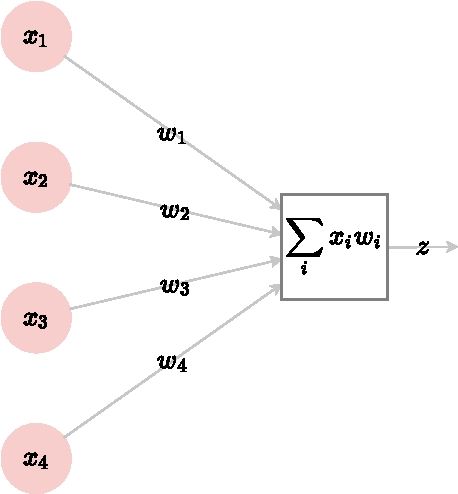
\includegraphics{media/images/perceptron.pdf}
\caption{Graphical representation of the
perceptron}\label{fig:perceptron}
\end{figure}

The perceptron learning algorithm constructs a weight vector \(\bm{w}\)
from a set of labelled training examples
\(\mathscr{X} = \{ (\bm{x}_0, y_0), \ldots, (\bm{x}_n, y_n) \}\) where
\(\bm{x}_i\) is the feature representation of the \(i\)-th training
example, and \(y_i\) is the true label of the example.

The following algorithm (Algorithm \ref{alg:perceptron-training}) is
used to learn a weight vector \(\bm{w}\) that correctly classifies all
examples on the training set (if possible, otherwise the algorithm fails
to terminate).

\begin{algorithm}[H]
\label{alg:perceptron-training}
\caption{Perceptron training}
\SetKwData{Converged}{converged}
\KwData{Training set: $\mathscr{X} = \{(\bm{x_0}, y_0), \cdots, (\bm{x_n}, y_n)\}$}
\KwResult{Binary classifier: $\bm{w} \cdot \bm{x} > 0$}
$\bm{w} \leftarrow \bm{0}$\;
\Converged $\leftarrow$ false\;
\While{\Converged = false}{
  \Converged $\leftarrow$ true\;
  \For{$i = 1$ to $|\mathscr{X}|$}{
    \If{$y_i \bm{w} \cdot \bm{x_i} \leq 0$}{
    $\bm{w} \leftarrow \bm{w} + \learningrate y_i \bm{x_i}$\;
    \Converged $\leftarrow$ false\;
    }
  }
}
\end{algorithm}

The idea is to iteratively build up a weight vector \(\bm{w}\) that
correctly classifies all training data. Initially starting with the zero
vector will result in the misclassification of all training examples as
they will all lie on the decision boundary, \(\bm{w} \cdot x = 0\). The
core of the algorithm depends on interpreting the dot product as a
measure of similarity. By adding weighted training feature vectors and
factoring in the correct sign of \(y_i\), \(\eta \bm{x}_i y_i\) to the
weight vector \(\bm{w}\), we increase the similarity of the updated
weight vector with the training example resulting in a more positive dot
product between \(\bm{w}\) and \(\bm{x}_i y_i\) which is more likely to
pass the decision threshold.

The perceptron learns a linear classifier, which is only of use if the
data is linearly separable, if it isn't then we have to consider
alternatives. Minsky and Papert used the following example
(fig.~\ref{fig:xor}) in
Perceptrons{[}\protect\hyperlink{ref-minsky1969_Perceptrons}{9}{]} to
demonstrate the limitations of a single perceptron, the figure shows the
function XOR where the red points cannot be separated from the green
points with a linear boundary, so a boundary like that shown in
fig.~\ref{fig:xor-non-linear-decision-boundary} is needed to separate
the data.

\begin{figure}
\centering
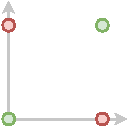
\includegraphics{media/images/xor.pdf}
\caption{XOR}\label{fig:xor}
\end{figure}

\begin{figure}
\centering
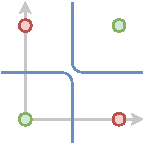
\includegraphics{media/images/xor-boundaries.pdf}
\caption{XOR with non linear decision
boundary}\label{fig:xor-non-linear-decision-boundary}
\end{figure}

Perceptrons can be used to learn a non linear decision boundary in two
ways. The first technique is to replace the dot product with a
\emph{kernel}, a function with properties similar to that of the dot
product. Use of a kernel as a replacement for the dot product can be
thought of as a transformation of the instances into a new space in
which a linear decision boundary is learnt. A kernel is chosen such that
it is likely that the data will be linearly separable in this new space.
Alternatively, the other technique is to stack perceptrons so that the
output of one is used as (one of) the input(s) to another, the network
formed is called a \emph{multilayer perceptron (MLP)}.

When using MLPs we have to adapt the perceptron's output to be followed
by a non-linear transformation \(\phi\); the reason for this is that if
we otherwise stack perceptrons without modification the network would
compute nested linear transformations which can be represented as a
single linear transformation, i.e.~MLPs without non linearity applied to
the output of each unit are no more expressive than a single perceptron;
the complexity of the decision boundaries learnt by MLPs is due to the
successive application of linear transformations and non linearities.

A small multi layer perceptron network is given in
fig.~\ref{fig:ann-example}. Each circle represents the body of a
perceptron in which the weighted sum of its inputs are calculated and
then passed through an activation function. Each edge between
perceptrons indicates the connectivity and weight between them. For
example, \(\neuron{1}{0}\) has two incoming connections from
\(\neuron{0}{0}\) with a weight \(+1\) and \(\neuron{0}{1}\) with a
weight \(0\), it will output the value
\({\phi\left(1 \cdot \neuron{0}{0} + 0 \cdot \neuron{0}{1})\right)}\)

\begin{figure}
\centering
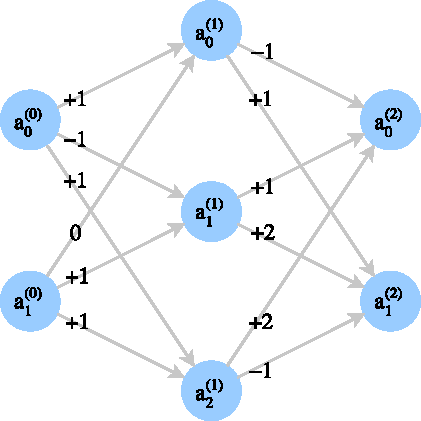
\includegraphics{media/images/ann-example.pdf}
\caption{Example Multilayer Perceptron with a single hidden
layer}\label{fig:ann-example}
\end{figure}

When producing any predictive model it is important to be able to
evaluate it to see whether it performs sufficiently well for its use
case. There are many measures to evaluate models including (but not
limited to): accuracy, precision, recall, and the \(F_1\) score; picking
a measure depends on the class ratio of the data you expect to run your
model on and the cost ratio that defines how costly it is to mistake one
class for another. Let's assume we've chosen accuracy to evaluate a
perceptron we've just trained, to evaluate it we could see how it
performs on the training data however since we know that the perceptron
perfectly splits the training data into two classes otherwise the
algorithm doesn't terminate the training accuracy will always be 100\%,
which makes this a useless test, instead we need a new dataset (perhaps
some data kept back from the training set) on which the model hasn't
been trained, referred to as the \emph{cross validation dataset}, on
which we evaluate the performance.

\textcolor{blue}{CHECK: Do you want me to add more about cross-fold validation etc?}\newline

\textcolor{green}{TODO: Talk about two feed forward methods}\newline

A forward pass of the network in fig.~\ref{fig:ann-example} is computed
using the activation function \({\phi(x) = \max(x, 0)}\) in
fig.~\ref{fig:ann-forward}. We traverse the graph from left to right,
computing the values of every perceptron in each layer before moving to
the next layer. The edges are relabelled with the product of the weight
and input to the edge, the diamonds below each perceptron show the sum
of the weighted inputs (the sum of the values labelled on the edges) and
the diamonds above show the output value of the perceptron after passing
the weighted sum of inputs through the activation function \(\phi\).

\begin{figure}
\centering
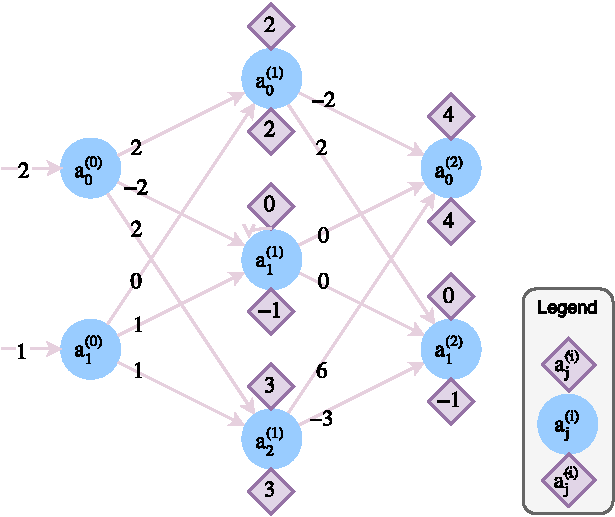
\includegraphics{media/images/ann-forward.pdf}
\caption{Forward propagation of the example ANN}\label{fig:ann-forward}
\end{figure}

To solve the XOR problem we can construct individual perceptrons that
simulate Boolean functions and then use the XOR propositional
decomposition (\(p \oplus q = (p \lor q) \land \lnot (p \land q)\)) to
construct a network that implements XOR, but this solution negates the
main benefit of using a learning algorithm in the first place: we want
the machine to form a solution.

Combining multiple perceptrons into a network forming a multi layer
perceptron brings us closer to the modern artificial neural network,
however we now have a new problem: learning the weights of all the
perceptrons. Since the weight vectors of the perceptrons in the network
are not independent, changing one will effect inputs deeper in the
network causing a change in the final output meaning we cannot use
Algorithm \ref{alg:perceptron-training}. An exhaustive search over the
weights of the perceptrons would be able to find an optimal weight
configuration, but would be computationally intractable due to the
combinatorial nature of the search.

Training multilayer perceptrons was the main impediment to their use
until the process of \emph{error back propagation} (first developed by
Kelley{[}\protect\hyperlink{ref-kelley1960_GradientTheoryOptimal}{10}{]}
and
Bryson{[}\protect\hyperlink{ref-dreyfus1990_Artificialneuralnetworks}{11}{]}{[}\protect\hyperlink{ref-schmidhuber2015_DeepLearningNeural}{12}{]})
was applied to the problem by Paul
Werbos{[}\protect\hyperlink{ref-schmidhuber2015_DeepLearningNeural}{12}{]}.
Back propagation gives us a tool to understand how modifying each
component of the weight vector of each perceptron changes the output of
the network. A loss function is defined that specifies how the output of
the network differs from the expected output, the partial derivatives of
the loss function with respect to each weight component
\(\frac{\partial a^{(n)}_i}{\partial w^{(l)}_j}\) are calculated. Having
obtained the partial derivatives we can perform gradient descent to
tweak the weights in such a way that the output of the network becomes
closer to the desired output for each training example, thereby
minimising the loss function.

The MLP is the foundation of modern neural networks, although in modern
parlance it is known as a \emph{fully connected feedforward network}.
The network is \emph{fully connected} since each neuron in layer
\(l + 1\) is connected to every neuron in layer \(l\). A
\emph{feedforward} network is one which neurons are connected in such a
way that no cycles are present (networks with cycles are known as
\emph{recurrent networks}).

\section{Convolutional neural networks
(CNNs)}\label{sec:background:cnns}

CNNs, a specialised form of ANNs, were first proposed in
{[}\protect\hyperlink{ref-fukushima1980_Neocognitronselforganizingneural}{13}{]}
as a network architecture called the \emph{neocognitron} inspired by the
research of Hubel and Wiesel on the visual
cortex{[}\protect\hyperlink{ref-hubel1959_Receptivefieldssingle}{14}{]}.
Hubel and Wiesel found that the neurons in the visual cortex of a cat's
brain responded to patterns in regions in the cats field of view, they
termed the region causing an excitation of a neuron as the
\emph{receptive field} of that neuron. Furthermore, they discovered that
neurons were arranged in such a way that neurons that had similar
receptive fields were also physically co-located in the cortex.
Fukushima \etal{} designed the connectivity of the neurons in the
neocognitron to model the connectivity of the neurons in the visual
cortex such that each neuron was connected to neurons in the previous
layer to form a receptive field. This architecture is very similar to
those currently in use.

Building on the work of the neocognitron, modern CNN models introduce
one substantial improvement: rather than learning parameters for each
individual neuron in a layer, we instead assume that there exist neurons
that fire in response to a class of patterns in the input for all
receptive fields, this allows us to learn only a single set of weights
to detect such patterns and effectively construct the neurons for each
receptive field at runtime. To implement this, convolutional filters are
learnt instead of individual neuronal weights which are then convolved
with the input tensor to produce the output.

The restricted architectures of CNNs facilitates a new view of these
networks compared to ANNs; the overarching theme is to raise the level
of abstraction from neurons to layers, and individual inputs to input
volumes. ANNs have no fixed/predetermined function, different groups of
neurons in a layer can serve different purposes, however this is not the
case in CNNs, layers are homogeneous in their function, e.g.~a
convolutional layer only computes convolution of its input. CNN
architectures are described by their constituent layers and the
hyperparameters that configure those layers, different layer types have
different hyperparameters.

Layers are constructed using this conceptual model and can be mapped
down to the traditional ANN model of neurons and weights.

Inputs and outputs from layers are thought of as tensors rather than
sets of disparate features encoded in a vector, this view is enabled the
homogeneity of the input. Typically for image and video processing
networks, the input is a 3D block, where width, \(W\), and height,
\(H\), correspond to the width and height of the input image, and the
depth, \(D\), of the block corresponds to the number of channels in the
image (e.g.~3 for RGB images, 1 for grayscale).

\subsection{Layers}\label{layers}

Layers can be thought of volume transformation functions, a volume of
dimensions \(W \times H \times D\) used as input by a layer is
transformed to an output volume of dimensions \(W' \times H' \times D'\)
where the new dimensions are a function of the input volume's dimensions
and layer's parameters.

There are many types of layers, but they mainly fit into four broad
categories: \emph{fully connected}, \emph{pooling},
\emph{convolutional}, \emph{activation}.

\subsubsection{Fully connected}\label{fully-connected}

Fully connected layers are like those in a MLP where each neuron is
connected to every neuron in the previous layer. These layers are very
large in parameters so are usually used further in the network when the
input volume size is considerably reduced. In CNNs, fully connected
layers draw together high level features from regions that are spatially
distant from each other, consider the task of detecting a bike in an
image, if you have filters that fire based on wheels, there will be
neurons that activate when wheels are present in different locations in
the image, the fully connected layer will be able to draw together the
wheel-neuron activations that are spatially separate and help
discriminate images of bikes from images with wheels that don't share
the same spatial relationship that wheels on bikes do.

\textcolor{blue}{CHECK: Dima, are the bike wheels a sensible example?}\newline

\subsubsection{Pooling}\label{pooling}

Pooling layers exist to increase the receptive field of deeper layers
enabling them to learn features than span larger spatial extents, this
is accomplished by reducing the size of the input volume by computing
some function over a region of the input yielding a single value,
usually this is a rectified linear computation \(\max(0, x)\) or
something similar like logistic regression.

\subsubsection{Convolutional}\label{convolutional}

Convolutional layers consist of one or more filters that are slid along
an input volume and convolved at each location producing a single value
which are aggregated in an output volume. The filter parameters are
learnt and are constant across different locations in the input volume,
this massively reduces the number of parameters of the model compared to
a fully connected layer handling similar volumes sizes making them much
more space efficient than fully connected networks.

The number of parameters in a convolutional layer is \emph{only}
dependent upon the filters. The filter is parameterised by its size,
stride and zero padding. The \emph{size} determines the volume of the
filter; \emph{stride}, how the filter is moved through the input volume;
\emph{zero padding}, whether or not the volume is padded with zeros when
convolved with the filter.

For a layer with 4 filters with the parameters:

\begin{itemize}
\tightlist
\item
  Size: \(W_f \times H_f \times D_f\) = \(4 \times 4 \times 3\)
\item
  Padding: \(W_p \times H_p \times D_p\) = \(0 \times 0 \times 0\)
\item
  Stride: \(S_w \times S_h \times S_d\) = \(1 \times 1 \times 0\)
\end{itemize}

The layer has a total of \(4 \cdot 4 \cdot 3 \cdot 1 \cdot 1 = 38\)
parameters.

\textcolor{green}{TODO: Expand on this with an example bank of filters and an
input volume and show to produce the output volume}\newline

\subsubsection{Activation}\label{activation}

\textcolor{green}{TODO: Add activation layer section}\newline

\subsection{Architectures}\label{architectures}

The architecture of a CNN refers to the choice of layers, and parameters
and connectivity of those layers. Architectures are designed to solve a
particular problem where the number of layers limits the complexity of
the features learnt by the network. Networks are designed such that they
have sufficient representational power (i.e.~number of layers, and
number of filters in those layers) necessary to learn the desired
mapping from input to output, but are as small as possible as each new
layer adds additional hyperparameters (number of filters, filter size,
stride size) to the network which further increases the already
considerable time spent searching for optimal hyperparameters by
training a network per hyperparameter configuration.

First we look at architectures for object detection as this task has
been the focus of most research inspiring architectures for action
recognition which we discuss afterwards.

\subsubsection{Object detection}\label{sec:background:object-detection}

Historically CNNs were extensively applied to the object detection
problem popularised by the ImageNet challenge
{[}\protect\hyperlink{ref-russakovsky2014_ImageNetLargeScale}{15}{]}.
The challenge consists of two main problems \emph{object detection} and
\emph{object localisation}, participants produce a model capable of
predicting the likelihood of object classes presence in a test image.
Models are evaluated based on their top-1 and top-5 error rate where the
top-\(N\) error rate is defined as the proportion of test images whose
prediction is considered an error if the ground truth label does not
appear in the top-\(N\) predictions.

\paragraph{AlexNet}\label{alexnet}

AlexNet{[}\protect\hyperlink{ref-krizhevsky2012_Imagenetclassificationdeep}{2}{]}
was the first CNN submission to ImageNet 2012 challenge achieving a
large error-rate reduction over previous state of the art methods
scoring a top-1 error rate of 36.7\% and top-5 error rate of 15.3\%.

\begin{figure}
\centering
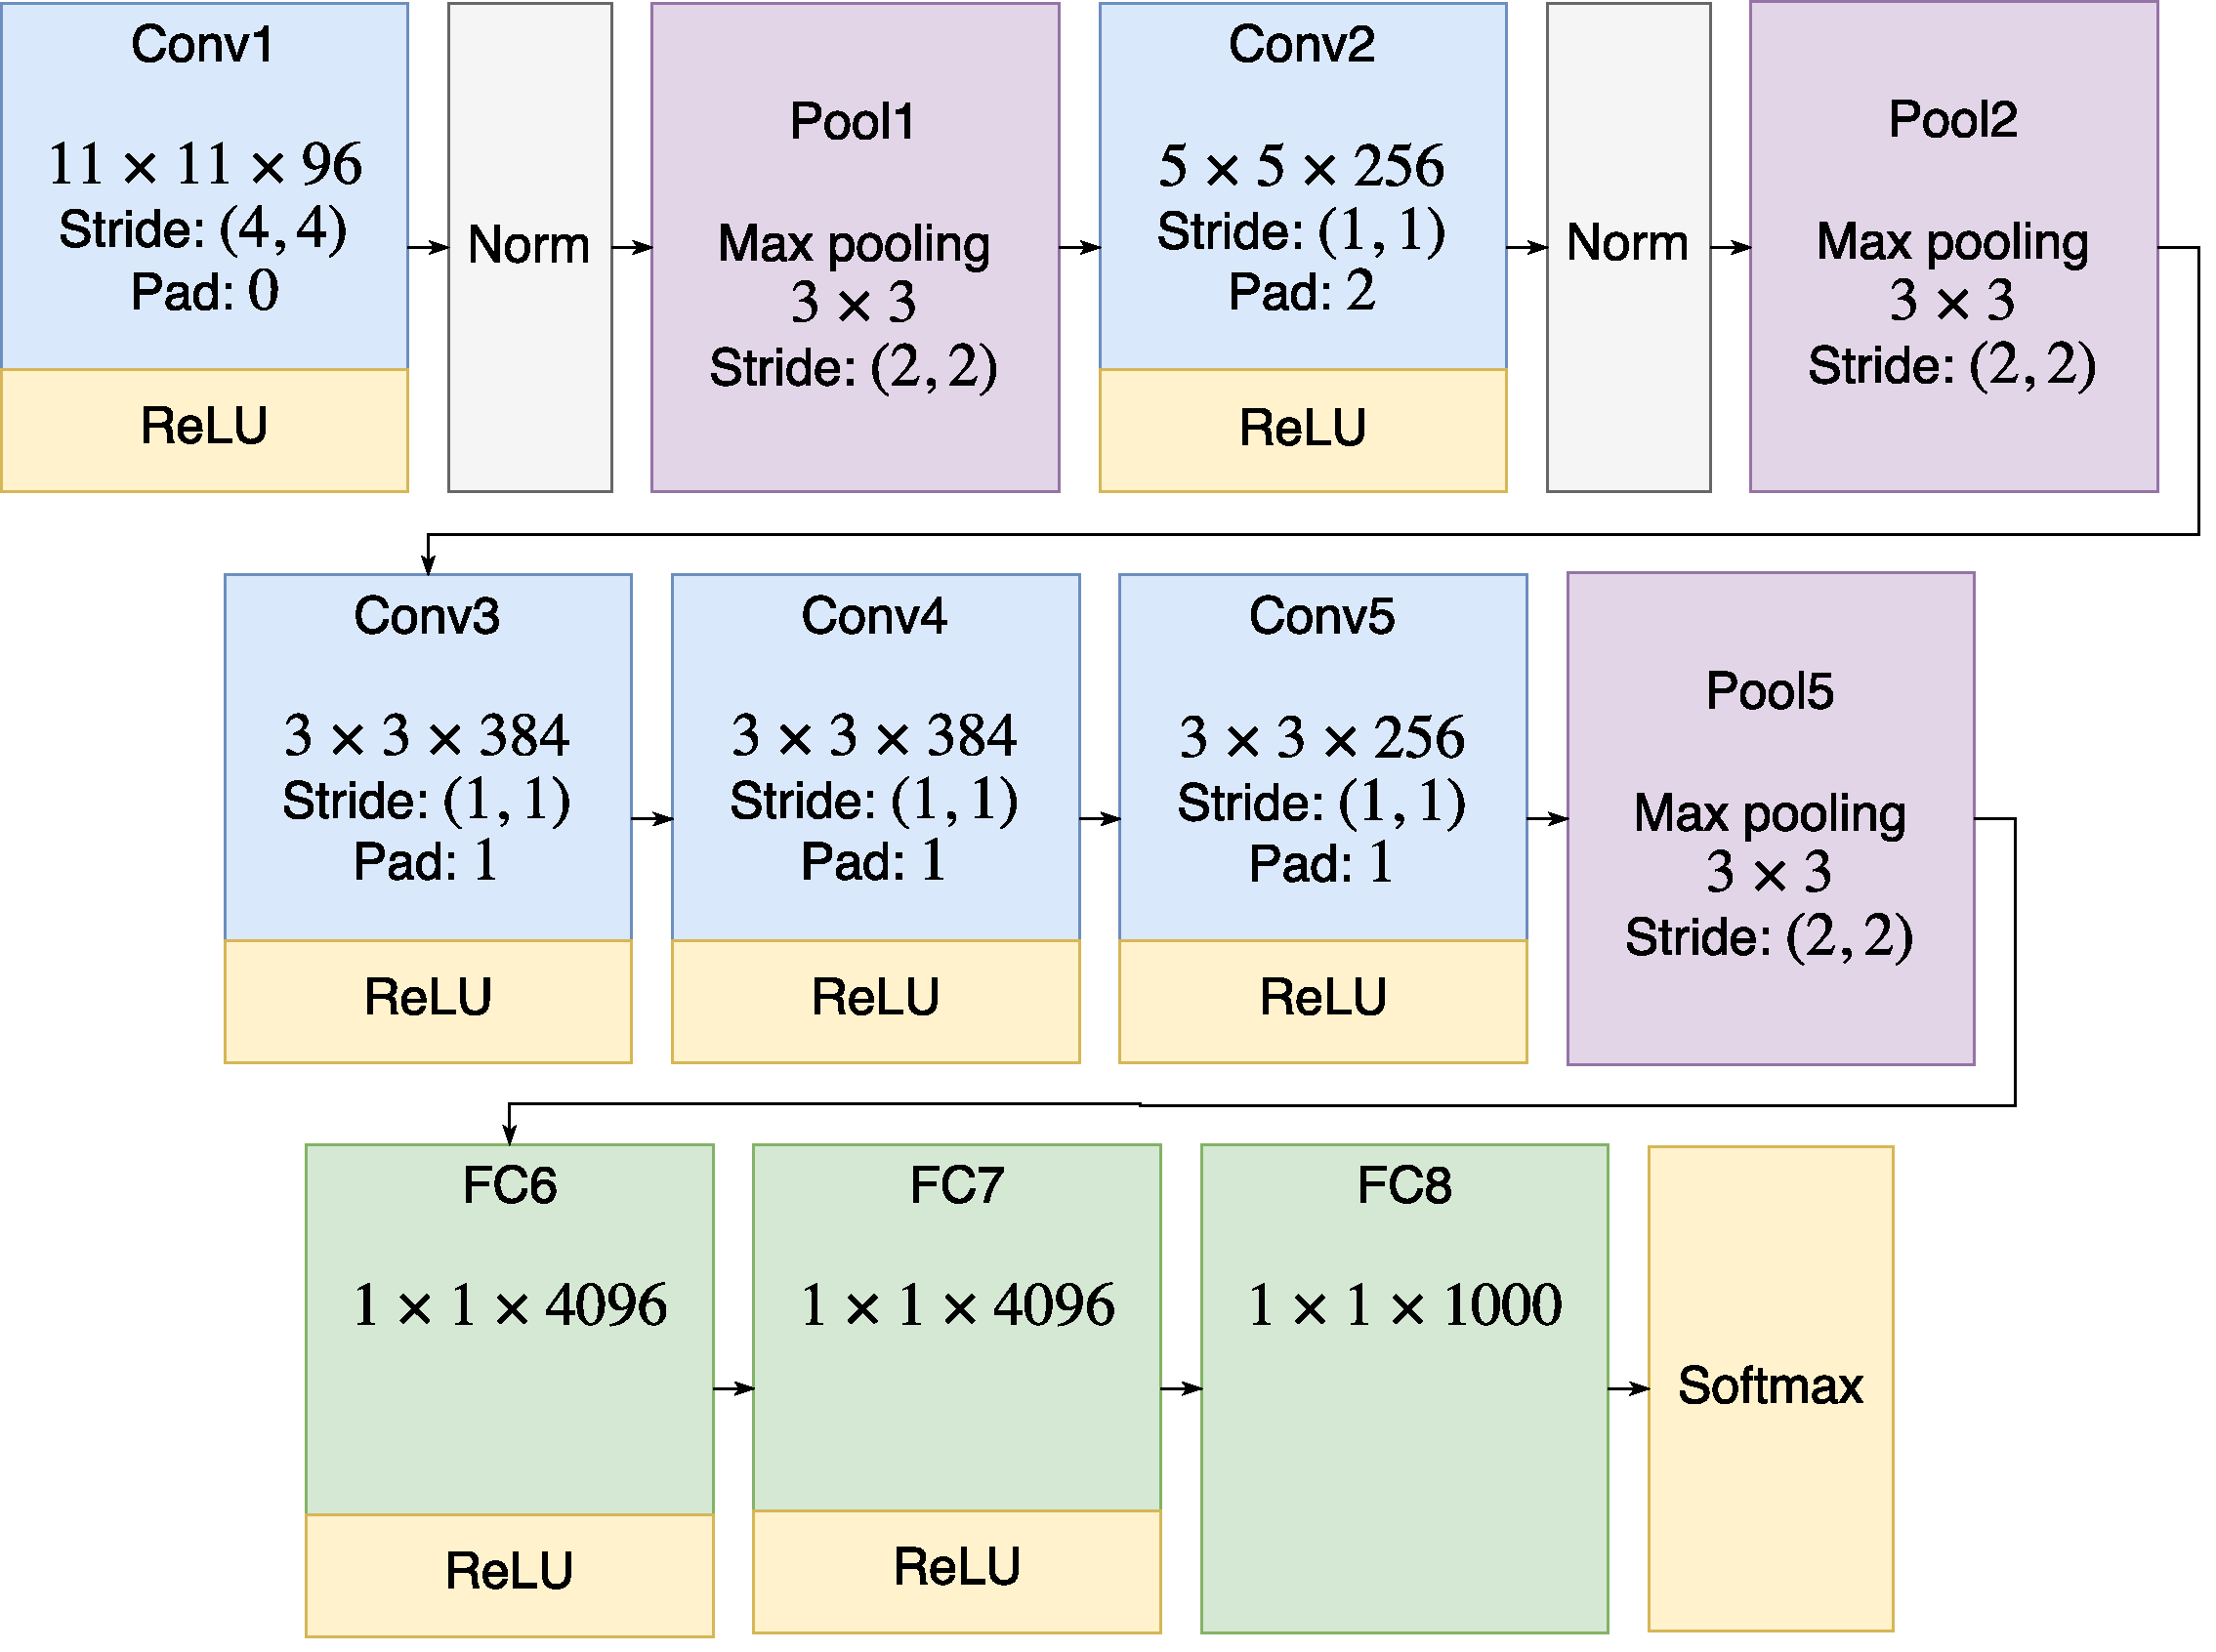
\includegraphics[height=2.00000cm]{media/images/alexnet.pdf}
\caption{AlexNet Architecture}\label{fig:architecture:alexnet}
\end{figure}

\paragraph{VGG16}\label{vgg16}

The VGG16 architecture
{[}\protect\hyperlink{ref-simonyan2014_VeryDeepConvolutional}{16}{]} was
developed as an enhancement over the original
AlexNet{[}\protect\hyperlink{ref-krizhevsky2012_Imagenetclassificationdeep}{2}{]}
architecture investigating the effects of using a `very deep'
architecture with many stacked convolutional layers. 6 similar network
architectures with increasing depth were trained and their
classification performance tested against the ImageNet dataset, the
network configurations with more convolutional layers performed better
than those with fewer resulting in two configuration VGG16 and VGG19
with 16 and 19 convolutional layers respectively. The VGG architectures
(used in an ensemble) won first place in the object classification
stream of the ImageNet 2014 challenge scoring a top-1 error rate of
24.4\% and top-5 error rate of 7.0\%, a considerable improvement over
AlexNet. Another deep network architecture by
Google{[}\protect\hyperlink{ref-szegedy2014_GoingDeeperConvolutions}{17}{]}
achieved similar error rates (second place) with 22 layers suggesting
that more layers isn't necessarily better, but that the architectures in
2012 were too shallow.

\begin{figure}
\centering
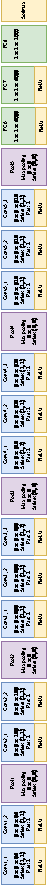
\includegraphics[width=2.00000cm,height=1.00000\textwidth]{media/images/vgg16-rotated90.pdf}
\caption{VGG16{[}\protect\hyperlink{ref-simonyan2014_VeryDeepConvolutional}{16}{]}
Architecture}\label{fig:architecture:vgg16}
\end{figure}

\subsubsection{Action recognition}\label{action-recognition}

\textcolor{green}{TODO: Start by introducing networks for action recognition from images e.g.
"Gkioxari contextual action recognition ICCV 2015"}\newline

The challenge of recognising actions from video sequences has recently
seen the application of CNNs inspired from their performance on object
detection. A variety of architectures for tackling the problem have
emerged which we shall explore in chronological order to see how
architectures have evolved over time ending with the current state of
the art.

The first investigation of CNNs for action recognition operating on raw
frame data (i.e.~without explicit feature extraction) was conducted in
{[}\protect\hyperlink{ref-baccouche2011_SequentialDeepLearning}{18}{]}.
They introduced an architecture with an input of a stack of video frames
which were then processed by multiple convolutional layers to learn
spatio-temporal features on the KTH human actions
dataset{[}\protect\hyperlink{ref-schuldt2004_Recognizinghumanactions}{19}{]}
the output of which was then used by a recurrent ANN called a long
short-term memory (LSTM) to obtain a prediction over the whole video
sequence, although they also compared classification with the LSTM layer
to a linear classifier and only found modest performance benefits (on
the order of a few percentage points) indicating that short clips from a
video may be sufficient for action recognition.

A similar architecture with a larger input volume was investigated in
{[}\protect\hyperlink{ref-ji2013_3DConvolutionalNeural}{20}{]}, instead
of training the whole network, the first layers were hand initialised to
obtain the following transformations: grayscale, spatial gradients in
both x and y directions, and optical flow in both x and y directions. A
video sequence processed by the first layer results in a stack of
grayscale video frames, spatial gradient frames and optical flow frames.
The network was evaluated on both the KTH dataset with competitive
performance to other methods developed at the time and
TRECVID{[}\protect\hyperlink{ref-_TRECVIDData}{21}{]} dataset improving
over the state of the art.

\begin{figure}
\centering
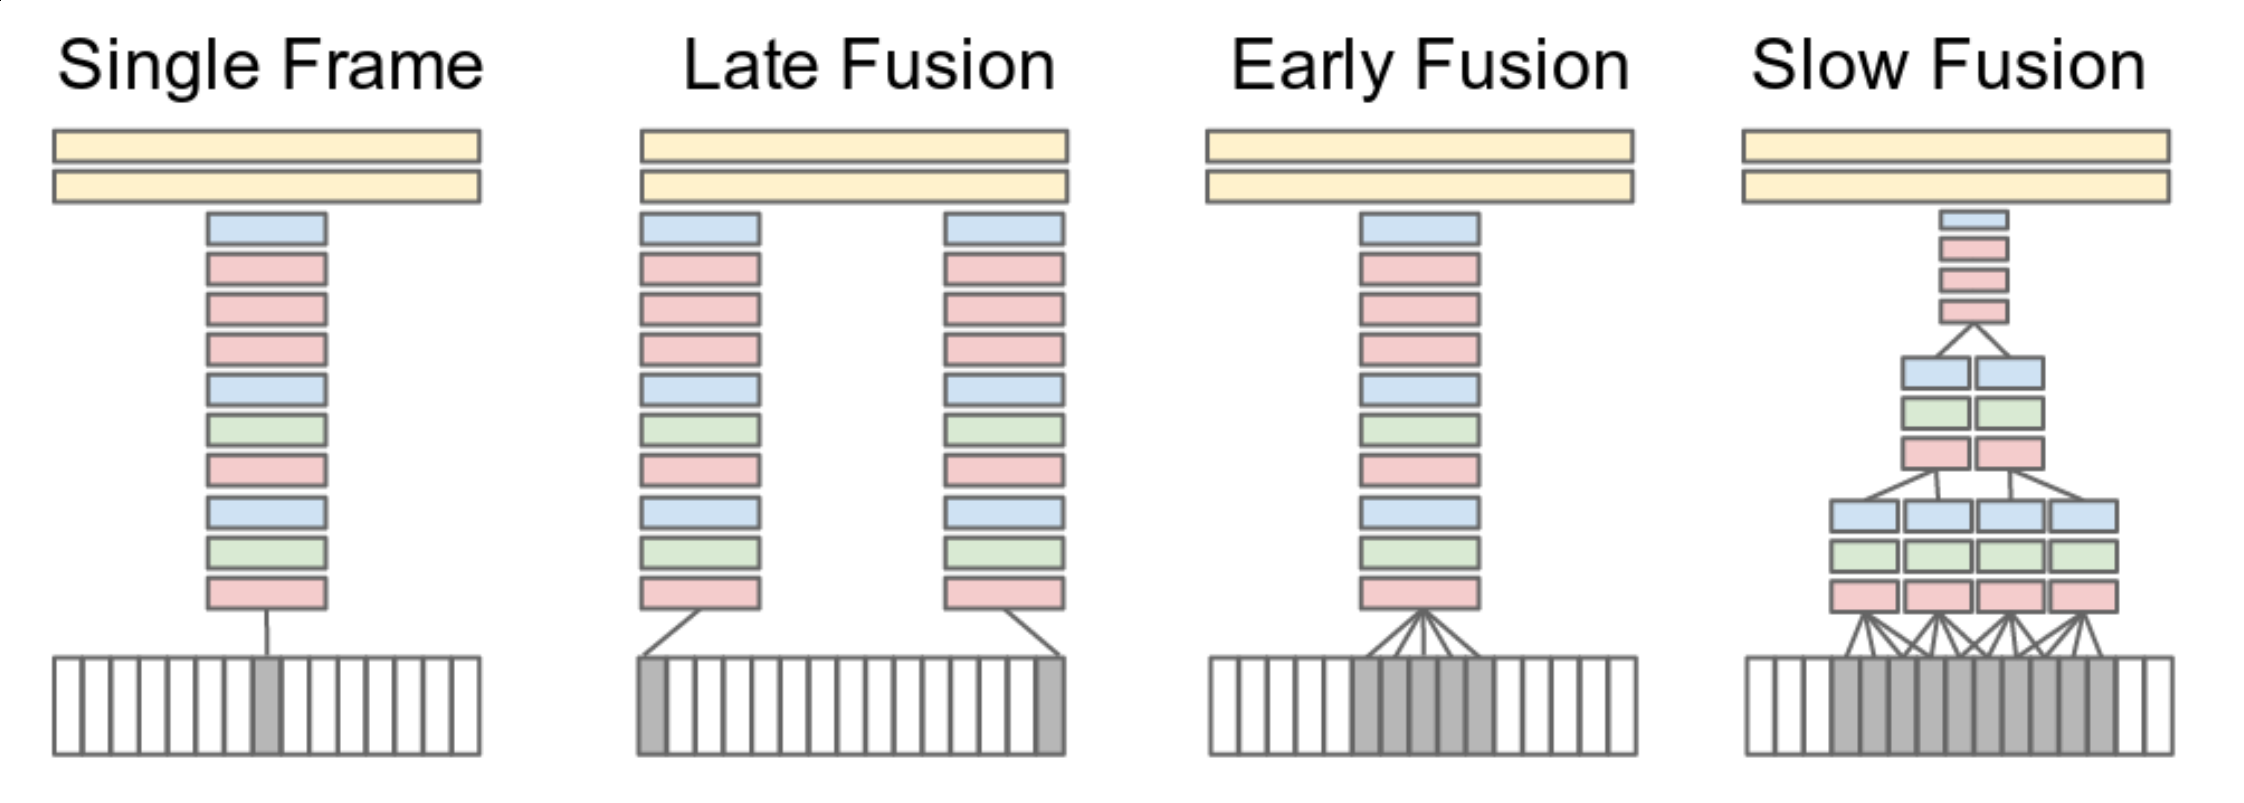
\includegraphics{media/images/karpathy2014-fusion-architectures.png}
\caption{CNN Architectures evaluated in
{[}\protect\hyperlink{ref-karpathy2014_LargeScaleVideoClassification}{22}{]}}\label{fig:karpathy2014-fusion-architectures}
\end{figure}

Investigations of different architectures for video classification were
performed in
{[}\protect\hyperlink{ref-karpathy2014_LargeScaleVideoClassification}{22}{]}.
Four different styles of architecture were investigated to determine
optimal stages of fusing temporal and spatial information. Each
architecture had a different connectivity to the video sequence stack,
from using a single frame as input to a dense sub-sequence of frames
(see fig.~\ref{fig:karpath2014-fusion-architectures} for architectures
and video sequence connectivity). Slow fusion, an architecture that
progressively enlarges the temporal and spatial field of view as the
input propagates deeper into the network performed best.

\textcolor{green}{TODO: expand on this}\newline

A biologically inspired architecture based on the two-stream visual
processing hypothesis is introduced in
{[}\protect\hyperlink{ref-simonyan2014_TwoStreamConvolutionalNetworks}{5}{]}.
The two stream hypothesis states that two processing streams are used in
the brain for processing visual input: the dorsal stream for motion,
good at detecting and recognising movements; and the ventral stream
recognising form, good at detecting objects. An architecture with two
streams based on the biological hypothesis is given, it has two streams,
the spatial for handling the appearance(analog of the ventral stream)
and the temporal for handling the motion(analog of the dorsal stream). A
video sequence is processed to obtain optical flow frames which are used
as input to the temporal stream, and a single frame is used as input to
the spatial stream. The two streams process the inputs in parallel each
of which produces an action prediction, the results are then combined
using a linear classifier.

In
{[}\protect\hyperlink{ref-feichtenhofer2016_ConvolutionalTwoStreamNetwork}{3}{]},
the authors extend the architecture presented in
{[}\protect\hyperlink{ref-simonyan2014_TwoStreamConvolutionalNetworks}{5}{]}
by observing that the previous architecture is incapable of matching
appearance in one sub-region to motion in another sub-region since each
stream is separate, to remedy this, the introduce a modified
architecture in which the two streams are combined after the last
convolutional layers resulting in a single spatio-temporal stream from
the fully connected layers onwards. The authors find that keeping the
spatial stream in addition to the spatio-temporal stream and combining
their respective predictions further increases performance over
predictions from the spatio-temporal stream alone.
\textcolor{green}{TODO: Report performance improvements over fusing into single tower}\newline

\textcolor{green}{TODO: split up the architectures discussed into those necessary for
background, and those for future work}\newline
\textcolor{green}{TODO: split out two stream cnn to separate section with detailed explanation}\newline
\textcolor{green}{TODO: move Karpathy 2014 to future work}\newline

\section{Video Datasets}\label{sec:background:datasets}

In sec.~\ref{sec:background:understanding} the surveyed papers
frequently make use of datasets, rather than explaining them as they are
referenced they are instead described and consolidated in this section.

\subsection{KTH - Human actions}\label{kth---human-actions}

The KTH human
action{[}\protect\hyperlink{ref-schuldt2004_Recognizinghumanactions}{19}{]}
dataset is composed of 6 action classes: walking, jogging, running,
boxing, hand waving and hand clapping performed by 25 subjects in 4
scenarios: outdoors, outdoors with scale variation, outdoors with
different clothes, and indoors. Each action class has 100 example clips

\begin{figure}
\centering
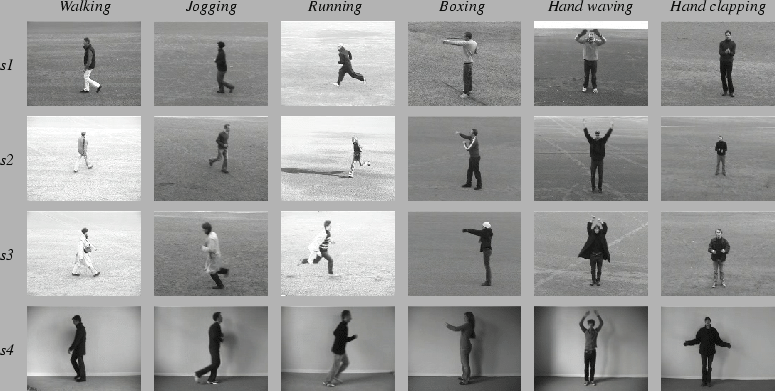
\includegraphics{media/images/kth-sample.png}
\caption{KTH Human
action{[}\protect\hyperlink{ref-schuldt2004_Recognizinghumanactions}{19}{]}
samples}
\end{figure}

\subsection{TRECVID - London Gatwick Airport Surveillance
video}\label{trecvid---london-gatwick-airport-surveillance-video}

TRECVID{[}\protect\hyperlink{ref-_TRECVIDData}{21}{]} is a competition
held each year by The National Institute of Standards and Technology. In
2008 one of the challenges held asked participants to detect 10
different events in 100 hours of CCTV camera footage shot inside London
Gatwick
Airport{[}\protect\hyperlink{ref-rose2009_TRECVid2008Event}{23}{]}. The
events to detect were: person puts mobile phone to ear; elevator doors
opening with a person waiting in front of them, but the person doesn't
get in before the doors close; someone drops or puts down an object;
someone moves through a controlled access door opposite to the normal
flow of traffic; one or more people walk up to one or more other people,
stop, and some communication occurs; when one or more people separate
themselves from a group of two or more people, who are either standing,
sitting , or moving together communicating, and then leaves the frame;
person running; person pointing; person taking a picture (descriptions
taken from {[}\protect\hyperlink{ref-rose2009_TRECVid2008Event}{23}{]}).

\subsection{Sports-1M - YouTube sport
actions}\label{sports-1m---youtube-sport-actions}

Sports-1M{[}\protect\hyperlink{ref-karpathy2014_LargeScaleVideoClassification}{22}{]}
is a weakly annotated action dataset obtained from YouTube consisting of
1 million videos over 487 sport classes. The videos are obtained by
searching for the sport class and then collecting videos from the search
results hence the labels in the dataset are noisy\footnote{There exists
  incorrect labelled examples in the dataset}.

\subsection{HMDB51 - Human motion
database}\label{hmdb51---human-motion-database}

HMDB51{[}\protect\hyperlink{ref-kuehne2011_HMDBlargevideo}{24}{]} is a
human activity dataset containing 6849 video clips over 51 action
classes each containing a minimum of 101 clips each fitting one of 5
broad categories: general facial actions, facial actions with object
manipulation, general body movements, body movements with object
interaction, body movements for human interaction. Examples are given in
fig.~\ref{fig:dataset:hmdb51:samples}\footnote{HMDB51 Samples image
  obtained from
  http://serre-lab.clps.brown.edu/resource/hmdb-a-large-human-motion-database/}

\begin{figure}
\centering
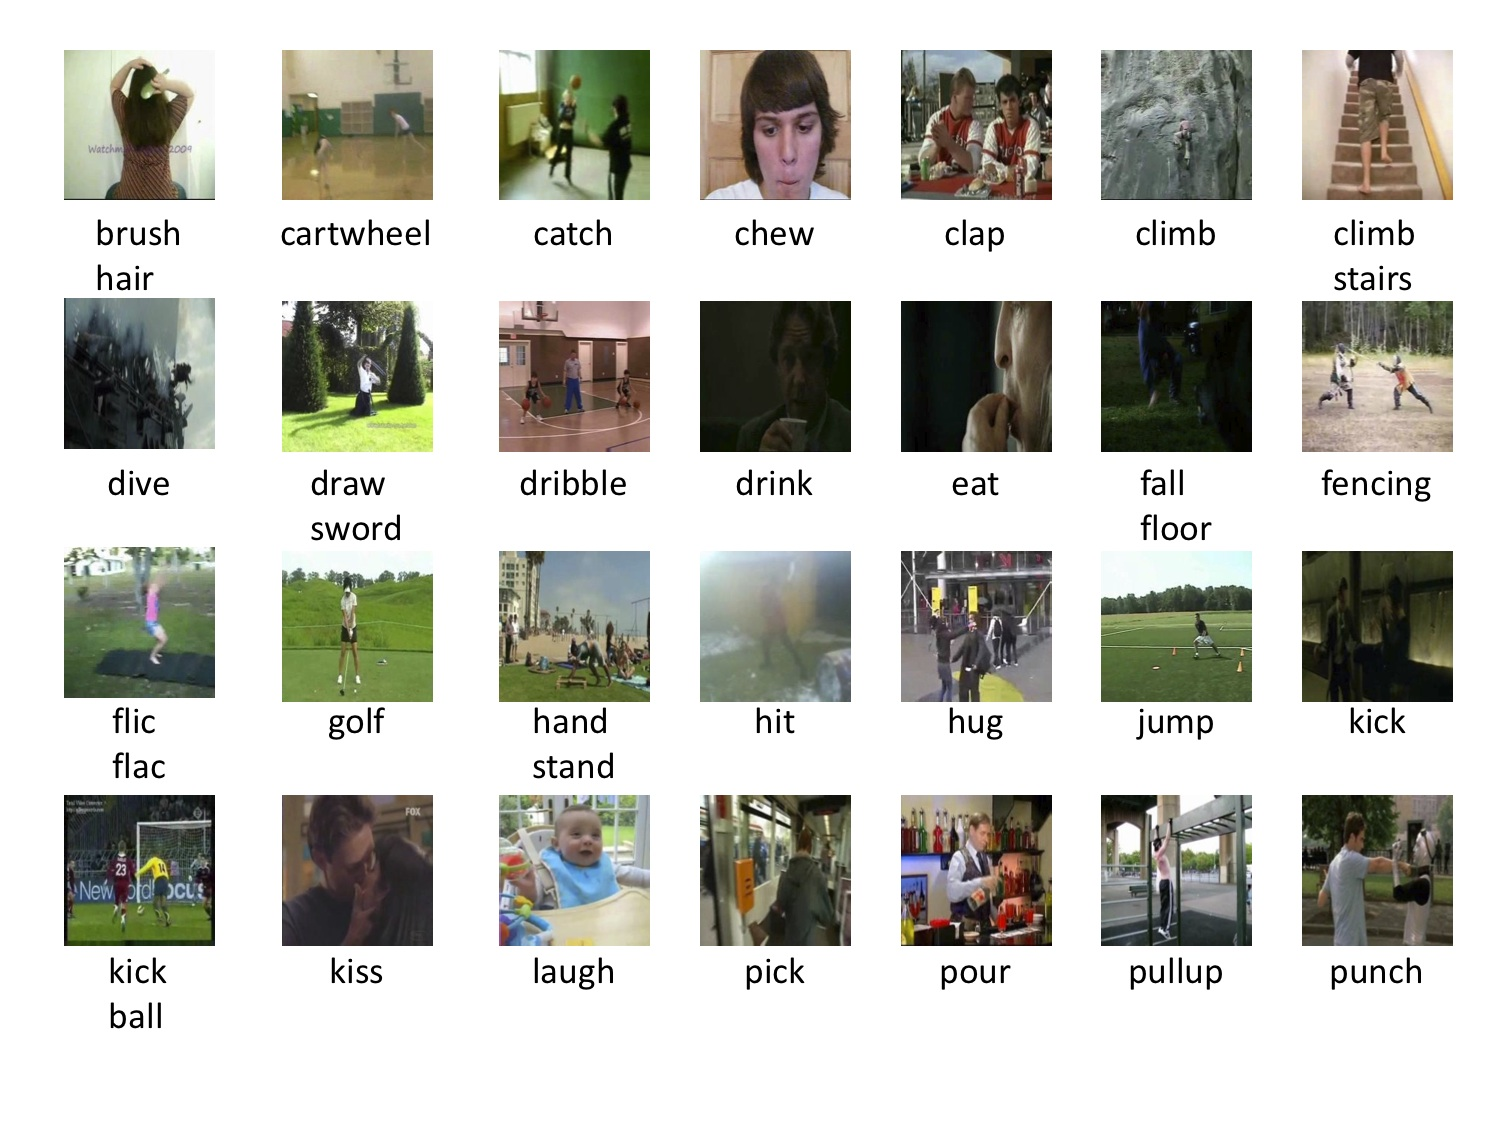
\includegraphics{media/images/hmdb51-sample.png}
\caption{HMDB51{[}\protect\hyperlink{ref-kuehne2011_HMDBlargevideo}{24}{]}
sample actions}\label{fig:dataset:hmdb51:samples}
\end{figure}

\subsection{UCF101 - Action
recognition}\label{ucf101---action-recognition}

UCF101{[}\protect\hyperlink{ref-soomro2012_UCF101Dataset101}{25}{]} is
an action dataset composed of 101 different actions across 5 broad
categories: human-object interaction, body-motion only, human-human
interaction, playing musical instruments, and sports. Each action class
has a minimum of 100 example clips associated with it. The dataset has a
diverse range of camera viewpoints, camera motion, object appearance and
pose, illumination conditions making it quite challenging compared to
some of the earlier datasets used for action recognition like KTH.

\begin{figure}
\centering
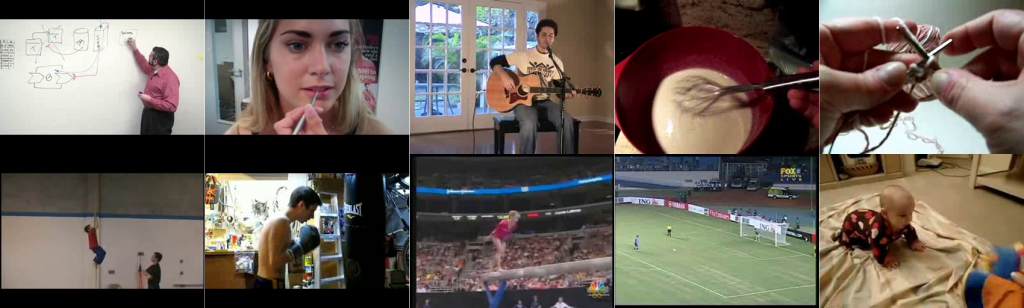
\includegraphics{media/images/ucf101-sample.png}
\caption{UCF101{[}\protect\hyperlink{ref-soomro2012_UCF101Dataset101}{25}{]}
sample actions}
\end{figure}

\subsection{BEOID - Bristol Egocentric Object Interaction
Dataset}\label{beoid---bristol-egocentric-object-interaction-dataset}

BEOID{[}\protect\hyperlink{ref-_BristolEgocentricObject}{26}{]} is an
human-object interaction dataset composed of videos shot from a head
mounted (egocentric) camera where the operator performs actions in one
of 6 different locations: kitchen, workspace, printer, corridoor with
locked door, cardiac gymn, and weight-lifting machine.

{[}BEOID{[}\protect\hyperlink{ref-_BristolEgocentricObject}{26}{]}
sample object interactions{]}{]}(media/images/beoid-sample.png)

\section{Understanding CNNs}\label{sec:background:understanding}

It is typical for CNNs to have on the order of \(10^7\)--\(10^8\)
parameters, with this complexity comes a difficulty in understanding how
the network works. There is a need to understand why a network correctly
classifies some examples but not others to aid the researcher in
determining higher performing architectures and problems in the dataset
or training process.

In
{[}\protect\hyperlink{ref-yosinski2015_UnderstandingNeuralNetworks}{28}{]},
Yosinski \etal{} identify that there are two main types of visualisation
methods developed for understanding the features learnt by CNNs:
network-centric and image-centric. Network-centric methods generate a
visualisation based on the trained network alone whereas image-centric
methods use an image or intermediate values computed in a forward pass
of the network from the image to generate a visualisation. Image-centric
visualisations help the researcher understand aspects like which areas
in the image contribute to the activation of a neuron. Network-centric
visualisations provide a more holistic visualisation of a neuron or
layer.

\textcolor{green}{TODO: expand on network-centric visualisations like filter visualisation}\newline

In
{[}\protect\hyperlink{ref-erhan2009_VisualizingHigherLayerFeatures}{29}{]},
Erhan \etal{} introduce the technique named \emph{activation
maximisation} for generating an artificial image to maximise the
activation of a chosen neuron by performing gradient ascent on an input
image. The technique is applied to a deep belief
network{[}\protect\hyperlink{ref-hinton2009_Deepbeliefnetworks}{30}{]}
(DBN) and a stacked denoising
autoencoder{[}\protect\hyperlink{ref-vincent2010_StackedDenoisingAutoencoders}{31}{]}
(SDAE) trained on the MNIST dataset of 60,000 hand written digits. They
found that neurons in the lower layers were activated by blobs and
patterns, and neurons in higher layers by actual images indicating that
the neurons have learnt higher level features from the combinations of
lower ones.

\textcolor{green}{TODO: Add figures explaining deconvolution}\newline
In
{[}\protect\hyperlink{ref-zeiler2013_VisualizingUnderstandingConvolutional}{32}{]},
Zeiler \& Fergus introduce two image-centric visualisations:
deconvolutional visualisation and occlusion studies. In deconvolutional
visualisation, an image is propagated through the network, the neuron
for visualisation is chosen and a deconvolutional
network{[}\protect\hyperlink{ref-zeiler2010_Deconvolutionalnetworks}{33}{]}
constructed from the network-under-analysis' weights is attached to the
layer in which the neuron of interest resides. All other neurons in the
layer of the chosen neuron are set to zero to produce a one-hot CNN code
which is used as input to the deconvolutional network that progressively
inverts the operation of the original network until the CNN code is
fully inverted back into an image. The resulting image retains aspects
of the original image in areas that contribute to the activation of the
chosen neuron. To invert a convolutional layer \(l_c\), a corresponding
convolutional layer \(l_c'\) is constructed in the deconvolutional
network where the filters from \(l\) are transposed in \(l_c'\) and the
input to \(l_c'\) is the output of \(l_c\). Rectified linear unit (ReLU)
layers are inverted by also applying ReLU, the idea being that a ReLU
layer ensures that the output of the layer is non negative, to preserve
this property that the output of a layer is non negative in the
deconvolutional network we too have to add a ReLU layer. Pooling layers
are inverted by recording the location in the filter from which the max
activation originated from, consider the following example: in a pooling
layer with \(2 \times 2\) filters, index each location in the filter by
\(i\), let \(i_{\text{max}}\) by the index of the location from which
the maximum value originates. When inverting the network, the value to
by distributed back to the \(2 \times 2\) grid is entirely given to
location \(i_{\text{max}}\).
\textcolor{green}{TODO: Reword explanation of deconv with diagrams}\newline

Simonyan \etal{} build on the work of Erhan \etal{} on activation
maximisation (a network-centric visualisation) by introducing
regularisation terms to the optimisation objective to improve the
interpretability of the generated image. The regularisation terms are
designed to restrict the generated image to the space of natural images,
since this is hard notion to express mathematically, the regularisation
terms act as proxy measures for how natural the synthesized image is. In
addition to improving the results of activation maximisation, it is
shown that the method is equivalent to the deconvolutional network
visualisation method proposed in
{[}\protect\hyperlink{ref-zeiler2013_VisualizingUnderstandingConvolutional}{32}{]}.
The authors also introduce a new image-centric visualisation method to
determine the contribution of individual pixels in an input image to its
classification by calculating the first order Taylor expansion of the
partial derivative of the predicted class neuron with respect to the
image space producing a linear function from which the weights of the
pixels approximate their relative importance in the classification.
These weights can then be visualised as a heatmap in the image space.

In
{[}\protect\hyperlink{ref-yu2014_VisualizingComparingConvolutional}{34}{]},
Yu \etal{} make a qualitative comparison between
AlexNet{[}\protect\hyperlink{ref-krizhevsky2012_Imagenetclassificationdeep}{2}{]}
and
VGG16{[}\protect\hyperlink{ref-simonyan2014_VeryDeepConvolutional}{16}{]}
using Deconvolutional visualisations of neurons in different layers,
they show that the deeper layers in VGG16 learn more discriminate
features than those in AlexNet.

\textcolor{blue}{CHECK: Possibly include Bach 2015?}\newline

Samek
\etal{}{[}\protect\hyperlink{ref-samek2015_Evaluatingvisualizationwhat}{35}{]},
{[}\protect\hyperlink{ref-samek2016_EvaluatingVisualizationWhat}{36}{]}
introduce a new image-centric visualisation method for determining why a
network made a classification decision, unlike activation maximisation,
the visualisation is based on the network's decision boundary rather
than a Taylor expansion about a particular image, a

\textcolor{green}{TODO: Need to read and understand the technique before I can explain it}\newline

Yosinski \etal{} explore a variety of priors/regularisers for use in the
activation maximisation visualisation of Erhan
{[}\protect\hyperlink{ref-erhan2009_VisualizingHigherLayerFeatures}{29}{]}
in
{[}\protect\hyperlink{ref-yosinski2015_UnderstandingNeuralNetworks}{28}{]}.
They release a toolbox named Deep Visualisation Toolbox\footnote{https://github.com/yosinski/deep-visualization-toolbox}
to observe live filter responses over arbitrary images on a user
provided CNN, furthermore the tool also facilitates deconvolutional
visualisation and activation maximisation.

Three methods are proposed in
{[}\protect\hyperlink{ref-mahendran2016_VisualizingDeepConvolutional}{37}{]}:
\emph{inversion}, inverting an arbitrary CNN code back to image space,
i.e.~synthesizing an image that produces a given CNN code;
\emph{activation maximisation}, new priors are proposed to improve
\emph{activation maximisation} (proposed by Erhan \etal{});
\emph{caricaturization} mutates a given image to exaggerate patterns to
further increase high activations in a layer of the network.

Nguyen \etal{} explore an image-centric probabilistic visualisation
method for determining the importance of regions in the input image to
maximise the activation of the neuron to produce a heatmap in
{[}\protect\hyperlink{ref-nguyen2016_Synthesizingpreferredinputs}{38}{]}.
To generate an excitation map for an image, the image is first processed
in a forward pass to determine the activations of all neurons in the
network, A prior distribution is defined to

Nguyen 2016: Synthesizing the preferred inputs for neurons
\textcolor{green}{TODO: Nguyen 2016}\newline

\textcolor{green}{TODO: rework section into taxonomy of visualisation techniques}\newline

\chapter{EBP}\label{ebp}

First a forward pass of the network is computed, this produces the
intermediate neuron values which are used as \emph{bottom up} salience
factors, then a probability distribution over the output layer is used
to specify \emph{top down} salience, then a excitation backprop pass
uses the probability distribution, intermediate neuron values and
weights to determine the probability of each intermediate neuron being a
winner at an arbitrary depth of the network.

Contrastive top down attention uses the insight that we're not only
interested in class we're localising, but also the absences of the other
classes (as classes may be correlated), we EBP the class of interest one
layer, then invert the output probability distribution, EBP one layer
and compute the difference between the two MWPs of the second last
layer, then EBP from there to the input.

\section{Example EBP calculation}\label{example-ebp-calculation}

We demonstrate EBP with a simple network composed of 5 neurons over 3
layers all using ReLU activations.

Notation:

\begin{itemize}
\tightlist
\item
  \(\neuron{i}{j}\) denotes the neuron with index \(j\) (0 indexed) in
  layer \(i\).
\item
  \(\weight{i}{j}{k}\) denotes the weight of the edge from neuron \(j\)
  in layer \(i\) to neuron \(k\) in layer \(i + 1\).
\item
  \(\neuroninput{i}{j}\) denotes the weighted sum of inputs to neuron
  \(j\) in layer \(i\)
\item
  \(\neuronoutput{i}{j}\) denotes the output of neuron \(j\) in layer
  \(i\)
\end{itemize}

\begin{equation}
\label{eq:neuron-input}
\neuroninput{i + 1}{j} = \sum_{a_{k}^{(i)} \in \children{i + 1}{j}} \weight{i}{k}{j} \neuronoutput{i}{k}
\end{equation}

\begin{equation}
\label{eq:neuron-output}
\neuronoutput{i}{j} = \phi(\neuroninput{i}{j})
\end{equation}

Where \(\phi\) is an activation, if not explicitly stated it is assumed
\(\phi(x) = \max(0, x)\) (ReLU activation).

At a high level, EBP consists of the following steps:

\begin{itemize}
\tightlist
\item
  Compute a forward pass of the network to determine the outputs of each
  neuron \(\neuronforward{i}{j}\)
\item
  Compute the scaling factors \(\ebpscalar{i}{j}\) of each neuron used
  in calculating the conditional winning probabilities of the children
  of that neuron.
\item
  Compute the conditional winning probabilities \(\cwp{i}{j}{i + 1}{k}\)
  of each neuron in the network.
\item
  Compute the winning probabilities of each neuron \(\mwp{i}{j}\) by
  computing the probability of each neuron and it's parents being
  winning neurons, then marginalising over the parent neurons.
\end{itemize}

\begin{equation}
\label{eq:ebp-cwp}
\cwp{i}{k}{i + 1}{j} = \begin{cases}
    \ebpscalar{i + 1}{j} \neuronforward{i}{k} \weight{i}{k}{j} & \weight{i}{k}{j} \geq 0 \\
    0 & \text{otherwise}
  \end{cases}
\end{equation}

\begin{equation}
\label{eq:ebp-cwp-scalar}
\ebpscalar{i + 1}{j} = 1 / \sum_{k:\weight{i}{k}{j} \geq 0} \neuronforward{i}{k} \weight{i}{k}{j}
\end{equation}

\begin{equation}
\label{eq:ebp-mwp}
\mwp{i}{k} = \sum_{\neuron{i+1}{j} \in \parents{i}{k}} \cwp{i}{k}{i + 1}{j} \mwp{i + 1}{j}
\end{equation}

Performing excitation backprop on the example network in
fig.~\ref{fig:ann-example}. The forward pass is detailed in
fig.~\ref{fig:ann-forward}.

First we define the input of the network (these could be any arbitrary
input):

\begin{align*}
\neuronforward{0}{0} &= 2\\
\neuronforward{0}{1} &= 1\\
\end{align*}

Now we compute the forward pass using the forward propagation rule

\textcolor{green}{TODO: move this to ANN section}\newline
\[\neuronforward{i}{k} = \phi(\sum_j \neuronforward{i - 1}{j} \cdot \weight{i - 1}{j}{k})\]

\begin{align*}
\neuronforward{1}{0} &= \max(0, \neuronforward{0}{0} \cdot \weight{0}{0}{0} +
    \neuronforward{0}{1} \cdot \weight{0}{1}{0})
  = max(0, (2 \cdot 1) + (1 \cdot 0)) = 2 \\
\neuronforward{1}{1} &= \max(0, (2 \cdot -1) + (1 \cdot 1)) = \max(0, -1) = 0\\
\neuronforward{1}{2} &= \max(0, (2 \cdot 1) + (1 \cdot 1)) = 3\\
\\
\neuronforward{2}{0} &= \max(0, \neuronforward{1}{0} \cdot \weight{1}{0}{0} +
    \neuronforward{1}{1} \cdot \weight{1}{1}{0} +
    \neuronforward{1}{2} \cdot \weight{1}{2}{0}) = 4 \\
\neuronforward{2}{1} &= \max(0, (2 \cdot 1) + (0 \cdot 2) + (3 \cdot -1)) = 0\\
\end{align*}

The next step is to compute the conditional winning probabilities of
each neuron given each parent neuron wins using eq.~\ref{eq:ebp-cwp}, to
compute this we need the scaling factors \(\ebpscalar{i}{j}\) which we
will compute first using eq.~\ref{eq:ebp-cwp-scalar} (in a computational
implementation these would be computed on a per layer basis and thrown
away once the layer values are calculated).

\begin{figure}
\centering
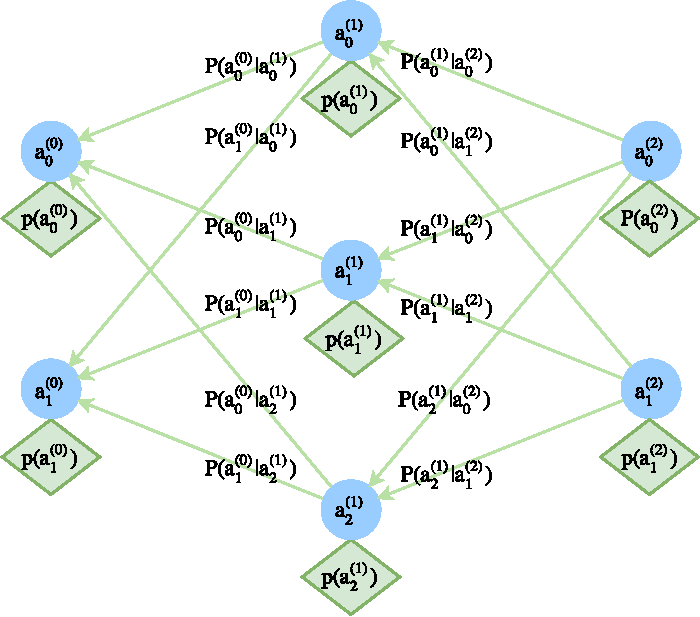
\includegraphics{media/images/ebp-example-mwp.pdf}
\caption{Flow of probabilities in EBP}
\end{figure}

\begin{figure}
\centering
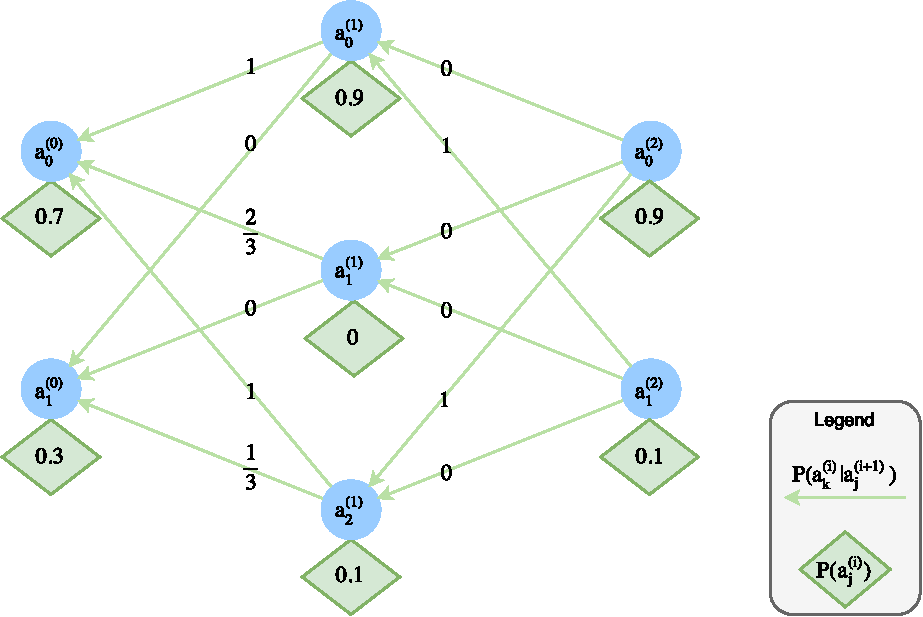
\includegraphics{media/images/ebp-example-mwp-concrete.pdf}
\caption{EBP CWP on the example network}
\end{figure}

\textcolor{green}{TODO: change legend to have $P(a_k^{(i)})$ in diamond}\newline

\begin{align*}
\ebpscalar{2}{0} &=
  \frac{1}{\left(\weight{1}{1}{0}\neuronforward{1}{1}\right) +
  \left(\weight{1}{2}{0} \neuronforward{1}{2}\right)}
  = \frac{1}{(1 \cdot 0) + (2 \cdot 3)}
  = \frac{1}{6}
  \\
\ebpscalar{2}{1} &= \frac{1}{(1\cdot 2) + (2 \cdot 0)} = \frac{1}{2}\\
\ebpscalar{1}{0} &= \frac{1}{
  \left(\weight{0}{0}{0} \neuronforward{0}{0}\right) +
  \left(\weight{0}{1}{0} \neuronforward{0}{0}\right)}
  = \frac{1}{(1 \cdot 2) + (0 \cdot 1)}
  = \frac{1}{2}
  \\
\ebpscalar{1}{1} &= \frac{1}{(1 \cdot 1)} = 1\\
\ebpscalar{1}{2} &= \frac{1}{(1 \cdot 2) + (1 \cdot 1)} = \frac{1}{3}\\
\end{align*}

Now for the conditional winning probabilities between layers 2 and 1:

\begin{align*}
\cwp{1}{0}{2}{0} &= 0 \\
\cwp{1}{0}{2}{1} &= \ebpscalar{2}{1} \neuronforward{1}{0} \weight{1}{0}{1} =
  \frac{1}{2} \cdot 2 \cdot 1 = 1
  \\
\cwp{1}{1}{2}{0} &= \ebpscalar{2}{0} \neuronforward{1}{1} \weight{1}{1}{0} =
  \frac{1}{6} \cdot 0 \cdot 1 = 0
  \\
\cwp{1}{1}{2}{1} &= \ebpscalar{2}{1} \neuronforward{1}{1} \weight{1}{1}{1} =
  \frac{1}{2} \cdot 0 \cdot 2 = 0
  \\
\cwp{1}{2}{2}{0} &= \ebpscalar{2}{0} \neuronforward{1}{2} \weight{1}{2}{0} =
  \frac{1}{6} \cdot 3 \cdot 2 = 1
  \\
\cwp{1}{2}{2}{1} &= 0\\
\end{align*}

Now layers 1 and 0:

\begin{align*}
\cwp{0}{0}{1}{0} &= \ebpscalar{1}{0} \neuronforward{0}{0} \weight{0}{0}{0} =
  \frac{1}{2} \cdot 2 \cdot 1 = 1\\
\cwp{0}{0}{1}{1} &= 0 \\
\cwp{0}{0}{1}{2} &= \frac{1}{3} \cdot 2 \cdot 1 = \frac{2}{3} \\
\cwp{0}{1}{1}{0} &= 0 \\
\cwp{0}{1}{1}{1} &= 1 \cdot 1 \cdot 1 = 1 \\
\cwp{0}{1}{1}{2} &= \frac{1}{3} \cdot 1 \cdot 1 = \frac{1}{3} \\
\end{align*}

We can now marginalise over the parent neurons in the conditional
winning probabilities if a prior distribution over the output neurons is
given to obtain the marginal winning probabilities of each neuron using
eq.~\ref{eq:ebp-mwp}.

Let's choose \(\mwp{2}{0} = 0.9\) and \(\mwp{2}{1} = 0.1\) for the prior
distribution. If we were investigating the saliency of a single neuron
we'd instead set the MWP of that neuron to 1 and the MWP of all other
neurons would be 0.

Marginalising over the parents of the hidden layer:

\begin{align*}
\mwp{1}{0} &= \sum_{\neuron{2}{j} \in \parents{1}{0}} \cwp{1}{0}{2}{j} \mwp{2}{j} \\
           &= \cwp{1}{0}{2}{0} \mwp{2}{0} + \cwp{1}{0}{2}{1} \mwp{2}{1} \\
           &= 0 \cdot 0.9 + 1 \cdot 0.1 = 0.1\\
\mwp{1}{1} &= 0 \cdot 0.9 + 0 \cdot 0.1 = 0\\
\mwp{1}{2} &= 1 \cdot 0.9 + 0 \cdot 0.1 = 0.9\\
\end{align*}

Finally to calculate the MWP of the input neurons to obtain the
posterior distribution:

\begin{align*}
\mwp{0}{0} &= 1 \cdot 0.1 + 0 \cdot 0 + \frac{2}{3} \cdot 0.9 = 0.7\\
\mwp{0}{1} &= 0 \cdot 0.1 + 1 \cdot 0 + \frac{1}{3} \cdot 0.9 = 0.3\\
\end{align*}

\chapter{Excitation backprop for temporal
networks}\label{sec:ebp-for-temporal-networks}

\textcolor{green}{TODO: Results from EBP on TSCNN trained on UCF101 and BEOID}\newline

\chapter{Future work}\label{sec:future-work}

\begin{itemize}
\tightlist
\item
  Applying activation maximisation on temporal networks with a prior
  encoding similarity over the multiple frames to generate videos.
\item
  Train DGN to invert temporal network to generate videos (like in
  {[}\protect\hyperlink{ref-nguyen2016_Synthesizingpreferredinputs}{38}{]})
\item
  Use deepdraw a la TSN paper to visualise actions of my networks
\end{itemize}

\chapter{Glossary}\label{glossary}

\begin{description}
\tightlist
\item[ANN]
Artificial Neural Network
\item[CNN]
Convolutional Neural Network
\item[DNN]
Deep artificial neural network (one with multiple hidden layers)
\item[EBP]
Excitation Backpropagation
\item[Top down attention]
Attention driven by top down factors like task information
\item[Bottom up attention]
Attention based on the salience of regions of the input image.
\item[Excitation Map]
A heat map over an image denoting the regions contributing contributing
to its classification
\end{description}

\chapter{Notation}\label{notation}

A full listing of all notation used.

\begin{description}
\item[\(\learningrate\)]
Learning rate (e.g.~see algorithm \ref{alg:perceptron-training})
\item[\(\neuron{l}{j}\)]
Neuron in layer \(l\) (0 indexed) at position \(j\) (0 indexed)
\item[\(\neuronforward{l}{j}\)]
The result of forward propagation at the neuron in layer \(l\) at
position \(j\)
\item[\(\weight{l}{j}{k}\)]
The weight connecting neuron \(\neuron{l}{j}\) to neuron
\(\neuron{l + 1}{k}\)
\item[\(\ebpscalar{l}{j}\)]
The scaling factor used in calculating the conditional probabilities in
EBP ensuring that the probabilities sum to one.
\item[\(\children{l}{j}\)]
The child neurons (those in layer \(l - 1\)) of the neuron in layer
\(l\) with index \(j\)
\item[\(\parents{l}{j}\)]
The parent neurons (those in layer \(l + 1\)) of the neuron in layer
\(l\) with index \(j\)
\item[\(\cwp{l}{j}{l + 1}{k}\)]
The \emph{conditional winning probability} of \(\neuron{l}{j}\) given
that \(\neuron{l + 1}{k}\) is winning neuron (see EBP).
\item[\(\mwp{l}{j}\)]
The \emph{marginal winning probability} of \(\neuron{l}{j}\) (see EBP)
\item[\(\neuroninput{l}{j}\)]
The input to neuron \(\neuron{l}{j}\).
\item[\(\neuronoutput{l}{j}\)]
The output of neuron \(\neuron{l}{j}\)
\end{description}

\chapter*{References}\label{references}
\addcontentsline{toc}{chapter}{References}

\hypertarget{refs}{}
\hypertarget{ref-ranasinghe2016_reviewapplicationsactivity}{}
{[}1{]} S. Ranasinghe, F. Al Machot, and H. C. Mayr, ``A review on
applications of activity recognition systems with regard to performance
and evaluation,'' \emph{International Journal of Distributed Sensor
Networks}, vol. 12, no. 8, p. 1550147716665520, Aug. 2016.

\hypertarget{ref-krizhevsky2012_Imagenetclassificationdeep}{}
{[}2{]} A. Krizhevsky, I. Sutskever, and G. E. Hinton, ``Imagenet
classification with deep convolutional neural networks,'' in
\emph{Advances in neural information processing systems}, 2012, pp.
1097--1105.

\hypertarget{ref-feichtenhofer2016_ConvolutionalTwoStreamNetwork}{}
{[}3{]} C. Feichtenhofer, A. Pinz, and A. Zisserman, ``Convolutional
Two-Stream Network Fusion for Video Action Recognition,'' Apr. 2016.

\hypertarget{ref-wang2016_TemporalSegmentNetworks}{}
{[}4{]} L. Wang \emph{et al.}, ``Temporal Segment Networks: Towards Good
Practices for Deep Action Recognition,'' Aug. 2016.

\hypertarget{ref-simonyan2014_TwoStreamConvolutionalNetworks}{}
{[}5{]} K. Simonyan and A. Zisserman, ``Two-Stream Convolutional
Networks for Action Recognition in Videos,'' Jun. 2014.

\hypertarget{ref-zhang2016_TopdownNeuralAttention}{}
{[}6{]} J. Zhang, Z. Lin, J. Brandt, X. Shen, and S. Sclaroff,
``Top-down Neural Attention by Excitation Backprop,'' Aug. 2016.

\hypertarget{ref-mcculloch1943_logicalcalculusideas}{}
{[}7{]} W. S. McCulloch and W. Pitts, ``A logical calculus of the ideas
immanent in nervous activity,'' \emph{Bulletin of Mathematical
Biophysics}, vol. 5, no. 4, pp. 115--133, Dec. 1943.

\hypertarget{ref-rosenblatt1957_Perceptronperceivingrecognising}{}
{[}8{]} F. F. Rosenblatt, ``The Perceptron: A perceiving and recognising
automaton (Project PARA),'' \emph{Cornell Aeronautical Laboratory},
1957.

\hypertarget{ref-minsky1969_Perceptrons}{}
{[}9{]} M. Minsky and S. Papert, \emph{Perceptrons}. Cambridge, MA: MIT
Press, 1969.

\hypertarget{ref-kelley1960_GradientTheoryOptimal}{}
{[}10{]} H. J. Kelley, ``Gradient Theory of Optimal Flight Paths,''
\emph{ARS Journal}, vol. 30, no. 10, pp. 947--954, 1960.

\hypertarget{ref-dreyfus1990_Artificialneuralnetworks}{}
{[}11{]} S. E. Dreyfus, ``Artificial neural networks, back propagation,
and the Kelley-Bryson gradient procedure,'' \emph{Journal of Guidance,
Control, and Dynamics}, vol. 13, no. 5, pp. 926--928, 1990.

\hypertarget{ref-schmidhuber2015_DeepLearningNeural}{}
{[}12{]} J. Schmidhuber, ``Deep Learning in Neural Networks: An
Overview,'' \emph{Neural Networks}, vol. 61, pp. 85--117, Jan. 2015.

\hypertarget{ref-fukushima1980_Neocognitronselforganizingneural}{}
{[}13{]} K. Fukushima, ``Neocognitron: A self-organizing neural network
model for a mechanism of pattern recognition unaffected by shift in
position,'' \emph{Biol. Cybernetics}, vol. 36, no. 4, pp. 193--202, Apr.
1980.

\hypertarget{ref-hubel1959_Receptivefieldssingle}{}
{[}14{]} D. H. Hubel and T. N. Wiesel, ``Receptive fields of single
neurones in the cat's striate cortex,'' \emph{J Physiol}, vol. 148, no.
3, pp. 574--591, Oct. 1959.

\hypertarget{ref-russakovsky2014_ImageNetLargeScale}{}
{[}15{]} O. Russakovsky \emph{et al.}, ``ImageNet Large Scale Visual
Recognition Challenge,'' Sep. 2014.

\hypertarget{ref-simonyan2014_VeryDeepConvolutional}{}
{[}16{]} K. Simonyan and A. Zisserman, ``Very Deep Convolutional
Networks for Large-Scale Image Recognition,'' Sep. 2014.

\hypertarget{ref-szegedy2014_GoingDeeperConvolutions}{}
{[}17{]} C. Szegedy \emph{et al.}, ``Going Deeper with Convolutions,''
Sep. 2014.

\hypertarget{ref-baccouche2011_SequentialDeepLearning}{}
{[}18{]} M. Baccouche, F. Mamalet, C. Wolf, C. Garcia, and A. Baskurt,
``Sequential Deep Learning for Human Action Recognition,'' in \emph{2nd
International Workshop on Human Behavior Understanding (HBU)}, 2011, pp.
29--39.

\hypertarget{ref-schuldt2004_Recognizinghumanactions}{}
{[}19{]} C. Schuldt, I. Laptev, and B. Caputo, ``Recognizing human
actions: A local SVM approach,'' in \emph{Proceedings of the 17th
International Conference on Pattern Recognition, 2004. ICPR 2004.},
2004, vol. 3, pp. 32--36 Vol.3.

\hypertarget{ref-ji2013_3DConvolutionalNeural}{}
{[}20{]} S. Ji, W. Xu, M. Yang, and K. Yu, ``3D Convolutional Neural
Networks for Human Action Recognition,'' \emph{IEEE Transactions on
Pattern Analysis and Machine Intelligence}, vol. 35, no. 1, pp.
221--231, Jan. 2013.

\hypertarget{ref-_TRECVIDData}{}
{[}21{]} ``TRECVID Data.'' {[}Online{]}. Available:
\url{http://trecvid.nist.gov/trecvid.data.html}. {[}Accessed:
14-Mar-2017{]}.

\hypertarget{ref-karpathy2014_LargeScaleVideoClassification}{}
{[}22{]} A. Karpathy, G. Toderici, S. Shetty, T. Leung, R. Sukthankar,
and L. Fei-Fei, ``Large-Scale Video Classification with Convolutional
Neural Networks,'' 2014, pp. 1725--1732.

\hypertarget{ref-rose2009_TRECVid2008Event}{}
{[}23{]} T. Rose, J. Fiscus, P. Over, J. Garofolo, and M. Michel, ``The
TRECVid 2008 Event Detection evaluation,'' in \emph{2009 Workshop on
Applications of Computer Vision (WACV)}, 2009, pp. 1--8.

\hypertarget{ref-kuehne2011_HMDBlargevideo}{}
{[}24{]} H. Kuehne, H. Jhuang, E. Garrote, T. Poggio, and T. Serre,
``HMDB: A large video database for human motion recognition,'' in
\emph{2011 International Conference on Computer Vision}, 2011, pp.
2556--2563.

\hypertarget{ref-soomro2012_UCF101Dataset101}{}
{[}25{]} K. Soomro, A. R. Zamir, and M. Shah, ``UCF101: A Dataset of 101
Human Actions Classes From Videos in The Wild,'' Dec. 2012.

\hypertarget{ref-_BristolEgocentricObject}{}
{[}26{]} ``Bristol Egocentric Object Interactions Dataset,''
\emph{data.bris}. {[}Online{]}. Available:
\url{http://data.bris.ac.uk/data/dataset/o4hx7jnmfqt01lyzf2n4rchg6}.
{[}Accessed: 16-Mar-2017{]}.

\hypertarget{ref-damen2014_DiscoveringTaskRelevant}{}
{[}27{]} D. Damen, T. Leelasawassuk, O. Haines, A. Calway, and W.
Mayol-Cuevas, ``Discovering Task Relevant Objects and their Modes of
Interaction from Multi-User Egocentric Video,'' 2014, pp. 30.1--30.13.

\hypertarget{ref-yosinski2015_UnderstandingNeuralNetworks}{}
{[}28{]} J. Yosinski, J. Clune, A. Nguyen, T. Fuchs, and H. Lipson,
``Understanding Neural Networks Through Deep Visualization,'' Jun. 2015.

\hypertarget{ref-erhan2009_VisualizingHigherLayerFeatures}{}
{[}29{]} D. Erhan, Y. Bengio, A. Courville, and P. Vincent,
``Visualizing Higher-Layer Features of a Deep Network.'' Jan-2009.

\hypertarget{ref-hinton2009_Deepbeliefnetworks}{}
{[}30{]} G. E. Hinton, ``Deep belief networks,'' \emph{Scholarpedia},
vol. 4, no. 5, p. 5947, May 2009.

\hypertarget{ref-vincent2010_StackedDenoisingAutoencoders}{}
{[}31{]} P. Vincent, H. Larochelle, I. Lajoie, Y. Bengio, and P.-A.
Manzagol, ``Stacked Denoising Autoencoders: Learning Useful
Representations in a Deep Network with a Local Denoising Criterion,''
\emph{The Journal of Machine Learning Research}, vol. 11, pp.
3371--3408, Mar. 2010.

\hypertarget{ref-zeiler2013_VisualizingUnderstandingConvolutional}{}
{[}32{]} M. D. Zeiler and R. Fergus, ``Visualizing and Understanding
Convolutional Networks,'' Nov. 2013.

\hypertarget{ref-zeiler2010_Deconvolutionalnetworks}{}
{[}33{]} M. D. Zeiler, D. Krishnan, G. W. Taylor, and R. Fergus,
``Deconvolutional networks,'' in \emph{2010 IEEE Computer Society
Conference on Computer Vision and Pattern Recognition}, 2010, pp.
2528--2535.

\hypertarget{ref-yu2014_VisualizingComparingConvolutional}{}
{[}34{]} W. Yu, K. Yang, Y. Bai, H. Yao, and Y. Rui, ``Visualizing and
Comparing Convolutional Neural Networks,'' Dec. 2014.

\hypertarget{ref-samek2015_Evaluatingvisualizationwhat}{}
{[}35{]} W. Samek, A. Binder, G. Montavon, S. Bach, and K.-R. Müller,
``Evaluating the visualization of what a Deep Neural Network has
learned,'' Sep. 2015.

\hypertarget{ref-samek2016_EvaluatingVisualizationWhat}{}
{[}36{]} W. Samek, A. Binder, G. Montavon, S. Lapuschkin, and K. R.
Müller, ``Evaluating the Visualization of What a Deep Neural Network Has
Learned,'' \emph{IEEE Transactions on Neural Networks and Learning
Systems}, vol. PP, no. 99, pp. 1--14, 2016.

\hypertarget{ref-mahendran2016_VisualizingDeepConvolutional}{}
{[}37{]} A. Mahendran and A. Vedaldi, ``Visualizing Deep Convolutional
Neural Networks Using Natural Pre-Images,'' \emph{International Journal
of Computer Vision}, vol. 120, no. 3, pp. 233--255, Dec. 2016.

\hypertarget{ref-nguyen2016_Synthesizingpreferredinputs}{}
{[}38{]} A. Nguyen, A. Dosovitskiy, J. Yosinski, T. Brox, and J. Clune,
``Synthesizing the preferred inputs for neurons in neural networks via
deep generator networks,'' May 2016.

\end{document}
